\documentclass{beamer}

\usepackage{beamerthemesplit}
\usepackage{graphicx}
\usepackage{color, natbib, hyperref}
\usepackage{multirow}
\usepackage{,array}
\newcolumntype{L}{>{\centering\arraybackslash}m{2.5cm}}
\usepackage{bibentry}
\nobibliography*

% define colors
\definecolor{jblue}  {RGB}{20,50,100}
\definecolor{ngreen} {RGB}{98,158,31}

%theme

\usetheme{boxes} 
%\usecolortheme{seahorse} 
\setbeamertemplate{items}[default] 
%\setbeamercovered{transparent}
\setbeamertemplate{blocks}[rounded]
\setbeamertemplate{navigation symbols}{} 
% set the basic colors
\setbeamercolor{palette primary}   {fg=black,bg=white}
\setbeamercolor{palette secondary} {fg=black,bg=white}
\setbeamercolor{palette tertiary}  {bg=jblue,fg=white}
\setbeamercolor{palette quaternary}{fg=black,bg=white}
\setbeamercolor{structure}{fg=jblue}
\setbeamercolor{titlelike}         {bg=jblue,fg=white}
\setbeamercolor{frametitle}        {bg=jblue!10,fg=jblue}
\setbeamercolor{cboxb}{fg=black,bg=jblue}
\setbeamercolor{cboxr}{fg=black,bg=red}

% reduce space before/after equations
\expandafter\def\expandafter\normalsize\expandafter{%
    \normalsize
    \setlength\abovedisplayskip{1pt}
    \setlength\belowdisplayskip{1pt}
    \setlength\abovedisplayshortskip{1pt}
    \setlength\belowdisplayshortskip{1pt}
}

% set colors for itemize/enumerate
\setbeamercolor{item}{fg=ngreen}
\setbeamercolor{item projected}{fg=white,bg=ngreen}

% set colors for blocks
\setbeamercolor{block title}{fg=ngreen,bg=white}
\setbeamercolor{block body}{fg=black,bg=jblue!10}

% set colors for alerted blocks (blocks with frame)
\setbeamercolor{block alerted title}{fg=white,bg=jblue}
\setbeamercolor{block alerted body}{fg=black,bg=jblue!10}
\setbeamercolor{block alerted title}{fg=white,bg=dblue!70} % Colors of the highlighted block titles
\setbeamercolor{block alerted body}{fg=black,bg=dblue!10} % Colors of the body of highlighted blocks

% set the fonts
\usefonttheme{professionalfonts}

\setbeamerfont{section in head/foot}{series=\bfseries}
\setbeamerfont{block title}{series=\bfseries}
\setbeamerfont{block alerted title}{series=\bfseries}
\setbeamerfont{frametitle}{series=\bfseries}
\setbeamerfont{frametitle}{size=\Large}
\setbeamerfont{block body}{series=\mdseries}
\setbeamerfont{caption}{series=\mdseries}
\setbeamerfont{headline}{series=\mdseries}


% set some beamer theme options
\setbeamertemplate{title page}[default][colsep=-4bp,rounded=true]
\setbeamertemplate{sections/subsections in toc}[square]
\setbeamertemplate{items}[circle]
\setbeamertemplate{blocks}[width=0.0]
\beamertemplatenavigationsymbolsempty

% Making a DAG
\usepackage{tkz-graph}  
\usetikzlibrary{calc}
\usetikzlibrary{shapes.geometric}
\usetikzlibrary{positioning}
\tikzstyle{VertexStyle} = [shape            = rectangle,
                               minimum width    = 6ex,%
                               draw]
 \tikzstyle{EdgeStyle}   = [->,>=stealth']      

% Define block styles
\tikzstyle{f} = [rectangle, draw, fill=blue!20, 
    text width=3em, text badly centered, node distance=1.75cm]
\tikzstyle{message} = [rectangle, draw, fill=green!20, 
    text width=3em, text centered]
\tikzstyle{io} = [draw, circle,fill=red!20, node distance=2cm,
    minimum height=2em]
\tikzstyle{line} = [draw, -latex']

% Math macros
\newcommand{\cD}{{\mathcal D}}
\newcommand{\cF}{{\mathcal F}}
\newcommand{\todo}[1]{{\color{red}{TO DO: \sc #1}}}

\newcommand{\reals}{\mathbb{R}}
\newcommand{\integers}{\mathbb{Z}}
\newcommand{\naturals}{\mathbb{N}}
\newcommand{\rationals}{\mathbb{Q}}

\newcommand{\ind}[1]{1_{#1}} % Indicator function
\newcommand{\pr}{\mathbb{P}} % Generic probability
\newcommand{\ex}{\mathbb{E}} % Generic expectation
\newcommand{\var}{\textrm{Var}}
\newcommand{\cov}{\textrm{Cov}}

\newcommand{\normal}{N} % for normal distribution (can probably skip this)
\newcommand{\eps}{\varepsilon}
\newcommand\independent{\protect\mathpalette{\protect\independenT}{\perp}}
\def\independenT#1#2{\mathrel{\rlap{$#1#2$}\mkern2mu{#1#2}}}

\newcommand{\convd}{\stackrel{d}{\longrightarrow}} % convergence in distribution/law/measure
\newcommand{\convp}{\stackrel{P}{\longrightarrow}} % convergence in probability
\newcommand{\convas}{\stackrel{\textrm{a.s.}}{\longrightarrow}} % convergence almost surely

\newcommand{\eqd}{\stackrel{d}{=}} % equal in distribution/law/measure
\newcommand{\argmax}{\arg\!\max}
\newcommand{\argmin}{\arg\!\min}


\mode<presentation>

\title[Simple Random Sampling: Not So Simple]{Simple Random Sampling: Not So Simple}
\author{Kellie Ottoboni \\ with Philip B.~Stark and Ron Rivest}
\institute[]{Department of Statistics, UC Berkeley\\Berkeley Institute for Data Science}
\date{BSTARS \\ March 23, 2017}

\begin{document}

\frame{
\titlepage
\vfill
\begin{columns}[T]
\begin{column}{.5\textwidth}
\begin{center}
\vspace{25pt}

\includegraphics[width=\textwidth]{fig/logo/dept1.pdf}
\end{center}
\end{column}
\begin{column}{.3\textwidth}
\begin{center}
\end{center}
\end{column}
\begin{column}{.3\textwidth}
\begin{center}

\includegraphics[width=0.9\textwidth]{fig/logo/BIDS.png}
\end{center}
\end{column}
\end{columns}
}



\section[Introduction]{Introduction}

\frame{
%\frametitle{Simple Random Sampling}
\textbf{Simple random sampling} lies at the heart of many statistical methods.
\vspace{20pt}

In practice, it is difficult to draw truly random samples.
\vspace{20pt}

Instead, people tend to draw samples using
\begin{enumerate}
\item A \textbf{pseudorandom number generator} (PRNG) that produces sequences of bits, plus
\item A sampling algorithm that maps a sequence of pseudorandom numbers into a subset of the population
\end{enumerate}
\vspace{20pt}

}



\frame
{
%  \frametitle{PRNGs}
  
  \textbf{Pseudorandom number generator:} a deterministic algorithm that produces sequences that are (ideally) computationally indistinguishable from the uniform distribution
  \vspace{20pt}

\begin{center}
\resizebox{10cm}{!}{    
\begin{tikzpicture}[node distance = 3cm, auto, scale = 0.5]
    % Place nodes
    \node[io] (seed) {Seed};
    \node [f, right of=seed, node distance = 3cm] (state) {Internal state};
    \node [message, right of=state, node distance = 3cm] (output) {Random bits};
    % Draw edges
    \path [line] (seed) -- (state);
    \path [line] (state) -- (output);
    \path (state) edge [->, in = 130, out = 50, distance = 20mm] node[above] {Update} (state);
    % Draw box 
    \draw ($(state.north west)+(-2.5,2.5)$)  rectangle ($(state.south east)+(2.5,-1)$);
\end{tikzpicture}
}
\end{center}

}
\frame{
%\frametitle{Pigeons and Pigeonholes}

%\begin{theorem}[Pigeonhole Principle]
%If there are $n$ pigeonholes and $m>n$ pigeons, then there exists at least one pigeonhole containing more than one pigeon.
%\end{theorem}
\begin{figure}[htbp]
\begin{center}
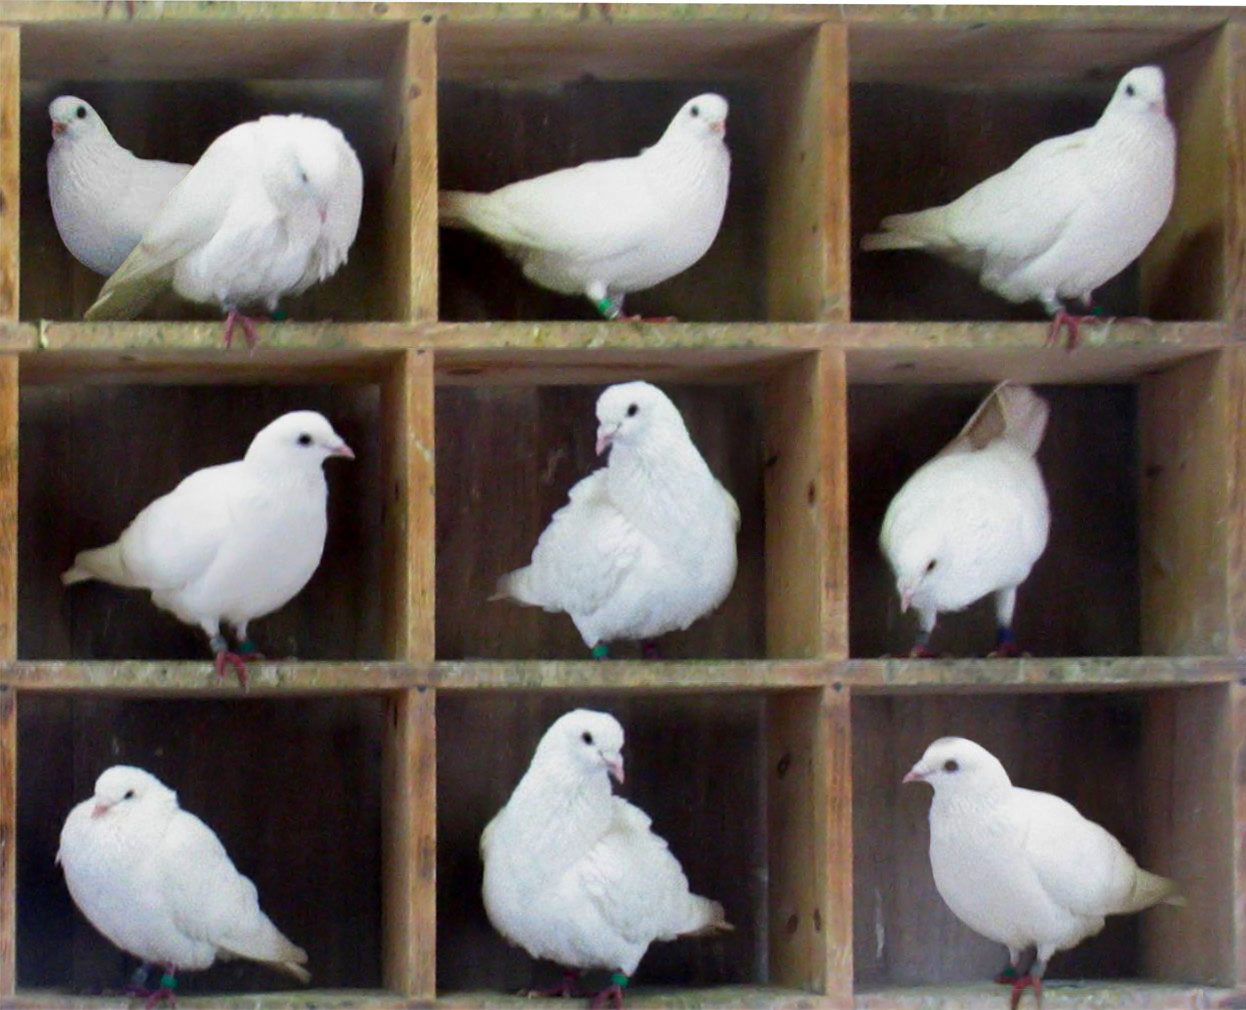
\includegraphics[width = .3\textwidth]{fig/TooManyPigeons.jpg}
\end{center}
\tiny \href{https://commons.wikimedia.org/w/index.php?curid=4658682}{(Wikipedia)}
\end{figure}

\begin{corollary}[Fewer pigeons than pigeonholes]
If the number of possible samples is greater than the size of a PRNG's state space, then the PRNG cannot possibly generate all samples.
\end{corollary}
}

\frame{
%\frametitle{Pigeons and Pigeonholes}

{\Large Does it matter in practice? }
%\pause
%
%\vspace{20pt}
%
%Period of 32-bit linear congruential generators (e.g. RANDU): $2^{32} \approx 4 \times 10^9$ \\
%Samples of size $10$ from $50$: ${50 \choose 10} \approx 10^{10}$ \\
%\textbf{More than half of samples cannot be generated}
%\vspace{20pt}
%\pause
%
%Period of Mersenne Twister (standard PRNG in Statistics): $2^{32 \times 624} \approx 2 \times 10^{6010}$ \\
%Permutations of $2084$ objects: $2084! \approx 3 \times 10^{6013}$\\
%\textbf{Less than $0.01\%$ of permutations can be generated}


\begin{center}
\begin{table}[htdp]
\begin{tabular}{LLLL}
PRNG & \# Internal states & \# Possibilities & Proportion of attainable possibilities \\
\hline
32-bit linear congruential generators & 4 billion & Samples of 10 out of 50 items $\approx 10$ billion & $0.4$ \\
\hline
Mersenne Twister & $\approx 2 \times 10^{6010}$ & Permutations of $2084$ items $\approx 3 \times 10^{6013}$ & $0.0001$
\end{tabular}
\end{table}%
\end{center}

%
%\begin{table}[htdp]
%\begin{center}
%\begin{tabular}{L|LL}
%PRNG & 32-bit linear congruential generators & Mersenne Twister\\
%\hline
% \# Internal states &4 billion &$\approx 2 \times 10^{6010}$\\
%\hline
% \# Desired samples &  Samples of 10 out of 50  $=$10 billion & Permutations of $2084$ objects $\approx 3 \times 10^{6013}$ \\
%\hline
% Ratio & $0.4$ &$0.0001$
%\end{tabular}
%\end{center}
%\label{default}
%\end{table}%

}



\frame{
%\frametitle{The good, the bad, and the ugly}



{\Large Even if a PRNG can generate all possible samples, it may not be sufficiently random. }


\vspace{20pt}


\begin{figure}[htbp]
\begin{center}
\includegraphics[width = 0.4\textwidth]{fig/randu.png} \\
\tiny \href{https://en.wikipedia.org/wiki/RANDU}{(Wikipedia)}
\end{center}

\vspace{20pt}
     $x_{n+1} = (65539 x_{n}) \mod 2^{31}$ \\
\vspace{10pt}
        {Triples of RANDU lie on 15 planes in 3D space.}
\end{figure}
}


\frame{
%\frametitle{A better alternative}

\textbf{One solution:} Find a class of PRNGs with infinite state space \textbf{and} good pseudorandom behavior


\begin{center}
\resizebox{10cm}{!}{    
\begin{tikzpicture}[node distance = 1cm, auto, scale = 0.5]
    % Place nodes
    \node [io] (IV) {IV};
    \node [f, right of=IV] (f1) {f};
    \node [f, right of=f1] (f2) {f};
%    \node [f, right of=f2, minimum width = 0cm, height = 0cm] (invisible) {};
    \node [f, right of=f2, node distance=3cm] (fn1) {f};
    \node [f, right of=fn1] (fend) {f};
%    \node [f, right of=invisible, node distance=3cm] (fend) {f};
    \node [f, right of=fend] (g) {g};
    \node [io, right of=g] (hx) {$h(x)$};
    \node [message, above of=f1] (m1) {$x_1$};
    \node [message, above of=f2] (m2) {$x_2$};
    \node [message, above of=fn1] (mn1) {$x_{n-1}$};
    \node [message, above of=fend] (mend) {$x_n$};
    \node [message, above right = of m1, above left = of mend, minimum width = 5cm] (message) {$x$};
    % Draw edges
    \path [line] (IV) -- (f1);
    \path [line] (f1) -- (f2);
    \path [line] (message) -- (m1);
    \path [line] (message) -- (m2);
    \path [line] (message) -- (mn1);
    \path [line] (message) -- (mend);
    \draw [-,dotted] (m2) -- (mn1);
    \path [line] (m1) -- (f1);
    \path [line] (m2) -- (f2);
     \path [line] (mn1) -- (fn1);
    \path [line] (mend) -- (fend);
    \path [line] (fend) -- (g);
    \path [line,dashed] (f2) -- (fn1);
    \path [line] (fn1) -- (fend);
    \path [line] (g) -- (hx);
\end{tikzpicture}
}
\end{center}


Cryptographic hash functions:
\begin{itemize}
\item computationally infeasible to invert
\item difficult to find two inputs that map to the same output
\item small input changes produce large, unpredictable changes to output
\item resulting bits are uniformly distributed
\end{itemize}

}


\frame{
%\frametitle{SHA256 in practice}


\begin{itemize}
\itemsep10pt
\item Preliminary results: SHA-256 hash function PRNG produces samples with equal probabilities while other common PRNGs don't
\item Replace the default PRNGs in Python
\url{https://www.github.com/statlab/cryptorandom}
\item Results apply more broadly to computer simulations: permutation tests, bootstrapping, MCMC, etc.
\end{itemize}

}

\begin{frame}
\frametitle{}
\begin{center}
\huge Thanks!
\vspace{20pt}

\normalsize
\url{https://github.com/kellieotto/prng-slides}
\end{center}
\end{frame}


\end{document}
